%% MODELO DE LATEX PARA TRABALHOS ACADÊMICOS

\documentclass[
	% -- opções da classe memoir --
	12pt,				% tamanho da fonte
	% openright,			% capítulos começam em pág ímpar (insere página vazia caso preciso)
    oneside,			% para impressão somente frente. Oposto a twoside (frente e verso)
	a4paper,			% tamanho do papel. 
	% -- opções da classe abntex2 --
	%chapter=TITLE,		% títulos de capítulos convertidos em letras maiúsculas
	%section=TITLE,		% títulos de seções convertidos em letras maiúsculas
	%subsection=TITLE,	% títulos de subseções convertidos em letras maiúsculas
	%subsubsection=TITLE,% títulos de subsubseções convertidos em letras maiúsculas
	% -- opções do pacote babel --
	english,			% idioma adicional para hifenização
	french,				% idioma adicional para hifenização
	spanish,			% idioma adicional para hifenização
	brazil,				% o último idioma é o principal do documento
	]{abntex2}


% ---
% PACOTES
% ---

% ---
% Pacotes fundamentais 
% ---
\usepackage{float}
\usepackage{csquotes}
\usepackage{cmap}				% Mapear caracteres especiais no PDF
\usepackage{lmodern}			% Usa a fonte Latin Modern
\usepackage[T1]{fontenc}		% Selecao de codigos de fonte.
\usepackage[utf8]{inputenc}		% Codificacao do documento (conversão automática dos acentos)
\usepackage{indentfirst}		% Indenta o primeiro parágrafo de cada seção.
\usepackage{color}				% Controle das cores
\usepackage{graphicx}			% Inclusão de gráficos
\usepackage{epigraph}
\usepackage{multicol}
\usepackage{multirow}
\usepackage{lipsum}				% para geração de dummy text
\usepackage[brazilian,hyperpageref]{backref}	 % Paginas com as citações na bibl
\usepackage[alf]{abntex2cite}	% Citações padrão ABNT



% --- 
% CONFIGURAÇÕES DE PACOTES
% --- 

% ---
% Configurações do pacote backref
% Usado sem a opção hyperpageref de backref
\renewcommand{\backrefpagesname}{Citado na(s) página(s):~}
% Texto padrão antes do número das páginas
\renewcommand{\backref}{}
% Define os textos da citação
\renewcommand*{\backrefalt}[4]{
	\ifcase #1 %
		Nenhuma citação no texto.%
	\or
		Citado na página #2.%
	\else
		Citado #1 vezes nas páginas #2.%
	\fi}%
% ---

% ---
% Informações de dados para CAPA e FOLHA DE ROSTO
% ---
\titulo{IDMATH}
\autor{Marielsom de Araújo Rocha}
\local{Picos - PI}
\data{5 de junho de 2017}
\instituicao{%
  Universidade Federal do Piauí
  \par
  Campus Senador Helvídio Nunes de Barros 
  \par
  Bacharelado em Sistemas de Informação}
\tipotrabalho{Relatório técnico}
% O preambulo deve conter o tipo do trabalho, o objetivo, 
% o nome da instituição e a área de concentração 
\preambulo{Trabalho de Conclusão de Curso em Bacharelado em Sistemas de Informação como requisito para a obtenção do grau de bacharel em Sistemas de Informação.}
% ---

% ---
% Configurações de aparência do PDF final

% alterando o aspecto da cor azul
\definecolor{blue}{RGB}{41,5,195}

% informações do PDF
\makeatletter
\hypersetup{
     	%pagebackref=true,
		pdftitle={\@title}, 
		pdfauthor={\@author},
    	pdfsubject={\imprimirpreambulo},
	    pdfcreator={LaTeX with abnTeX2},
		pdfkeywords={abnt}{latex}{abntex}{abntex2}{relatório técnico}, 
		colorlinks=true,       		% false: boxed links; true: colored links
    	linkcolor=blue,          	% color of internal links
    	citecolor=blue,        		% color of links to bibliography
    	filecolor=magenta,      		% color of file links
		urlcolor=blue,
		bookmarksdepth=4
}
\makeatother
% --- 


% ---
% compila o indice
% ---
\makeindex
% ---







% ----
% Início do documento
% ----
\begin{document}

% Retira espaço extra obsoleto entre as frases.
\frenchspacing 

% ----------------------------------------------------------
% ELEMENTOS PRÉ-TEXTUAIS
% ----------------------------------------------------------
% \pretextual

% ---
% Capa
% ---
\imprimircapa
% ---

% ---
% Folha de rosto
% (o * indica que haverá a ficha bibliográfica)
% ---
\imprimirfolhaderosto*
% ---






% ---
% Agradecimentos
% ---
\begin{agradecimentos}
Insira seus agradecimentos aqui.
\end{agradecimentos}
% ---

% ---
% Epigrafe
% ---
\vspace*{\fill}
{ \raggedleft
	\textit{A tarefa não é tanto ver aquilo que ninguém viu, mas pensar o que ninguém ainda pensou sobre aquilo que todo mundo vê. \\
		Arthur Schopenhauer}
	~
}
\pagebreak


% ---
% RESUMO
% ---

% resumo na língua vernácula (obrigatório)
\begin{resumo} %% AQUI COMEÇA A PÁGINA DE RESUMO
 

 
 % No Resumo precisa ser um pouco mais abrangente mantendo a objetividade das linhas já escritas.

 \vspace{\onelineskip}
    
 \noindent
 \textbf{Palavras-chaves}: latex. abntex. editoração de texto.
\end{resumo} %AQUI TERMINA A PÁGINA DE RESUMO


\begin{resumo}[Abstract]

  
    
\end{resumo}


% ---
% inserir lista de ilustrações
% ---

\listoffigures* %% o * indica que não será incluso no sumário
\cleardoublepage %% Pula página
% ---

% ---
% inserir lista de tabelas
% ---

\listoftables*
\cleardoublepage
% ---

% ---
% inserir lista de abreviaturas e siglas
% ---
\begin{siglas}
  \item[Fig.] Area of the $i^{th}$ component
  \item[456] Isto é um número
  \item[123] Isto é outro número
  \item[lauro cesar] este é o meu nome
\end{siglas}
% ---

% ---
% inserir lista de símbolos
% ---
\begin{simbolos}
  \item[$ \Gamma $] Letra grega Gama
  \item[$ \Lambda $] Lambda
  \item[$ \zeta $] Letra grega minúscula zeta
  \item[$ \in $] Pertence
\end{simbolos}
% ---

% ---
% inserir o sumario
% ---

\tableofcontents*

% ---

% ----------------------------------------------------------
% ELEMENTOS TEXTUAIS  (necessário para incluir número nas páginas)
% ----------------------------------------------------------
\textual


% ----------------------------------------------------------
% Introdução
% ----------------------------------------------------------
\chapter{Introdução} %% NOVO CAPÍTULO (REPARE QUE ELE AUTOMATICAMENTE JÁ COLOCA O NÚMERO DO CAPÍTULO E JÁ ADICIONA NO SUMÁRIO)

Escolher uma área acadêmica é um dos principais desafios para a maior parte dos jovens, pois além da indecisão que alguns possuem para a escolha profissional, eles também se sentem influenciados pelos familiares, amigos e até mesmo por questões financeiras, motivando-os a tomar uma decisão que pode ou não ser adequada para sua carreira \cite{goncalves}.

O processo de orientação vocacional é uma das formas de auxiliar os alunos que estão concluindo o ensino médio ou já o concluíram. Uma das dificuldades é que no Brasil, a maior parte das instituições de ensino não possuem psicólogos.

Uma pesquisa realizada por graduandos da Universidade Federal Fluminense (UFF), nas cidades de Niterói, Itaboraí, São Gonçalo e Rio de Janeiro, apontou que dentre as 65 das instituições públicas e privadas visitadas, apenas 15\% delas possuem psicólogos. Diante dos dados apresentados, podemos observar a grande escassez destes profissionais \cite{arreguy}.

Uma outra alternativa seria o auxílio dos professores na busca do desenvolvimento e maturação vocacional de cada aluno. Contudo, é uma tarefa complicada pois requer tempo e esforço para identificar o perfil de cada estudante e mostrar para eles áreas correlacionadas, por esse motivo, o teste vocacional é um dos meios de auxílio em que a maior parte dos discentes podem recorrer \cite{marielsom}.

"Os testes vocacionais tinham a finalidade de orientar profissionalmente os jovens para uma escolha coerente com suas aptidões" \cite{abade}, o questionário é uma das formas que os testes são disponibilizados e são elaborados por profissionais da área de psicologia, tem por objetivo avaliar, analisar, esclarecer e informar o examinando suas áreas de interesses, aptidões específicas e gerais, que se apresentam inseridas em suas possibilidades.

A falta de orientação vocacional acarreta vários pontos negativos, um deles é o alto grau de desistência. Uma pesquisa levantada pela Universidade Estadual de Montes Claros – MG com estudantes do Curso de Ciências Contábeis, entres os anos de 2004 à 2008, apontou que dos 45 entrevistados, 16\% deles desistiram por falta de orientação vocacional \cite{evasao}.


As citações de trabalhos referenciados deverá ser assim: \cite{f1}.


\begin{table}[hbt] %% EXEMPLO DE TABELA FEITA POR MEIO DO http://www.tablesgenerator.com/
\begin{center}
\caption{Exemplo de Tabela.} %% LEGENDA (REPARE QUE ELE JÁ COLOCA A NUMERAÇÃO AUTOMATICAMENTE E JÁ ADICIONA À LISTA DE TABELAS
\begin{tabular}{|l|l|lll}
\cline{1-2}
Produto & Valor   &  &  &  \\ \cline{1-2}\cline{1-2}
sdadasd & asdasd  &  &  &  \\ \cline{1-2}
asdasd  & asasdas &  &  &  \\ \cline{1-2}
dsad    & asdas   &  &  &  \\ \cline{1-2}
\end{tabular}
\end{center}
\end{table}


Inserir texto.....
A seguir você encontrará um exemplo de Figura. No texto referencie-a assim: Figura \ref{figura1}.



\section{Contextualização do problema}

Inserir texto...


\section{Objetivo}


O objetivo deste trabalho...



\section{Organização do Trabalho}
Este trabalho está organizado em 6 (seis) capítulos. Iniciando com o Referencial Teórico, onde é apresentada a discalculia, bem como suas características, métodos de intervenção, formas de como a tecnologia pode ser uma ferramenta fundamental no diagnóstico destas crianças. No capítulo 3 (três), os trabalhos semelhantes a este. No capítulo 4 (quatro)  faz-se a apresentação do software, apontando seus aspectos e comportamentos. 5 (cinco) testes e resultados e no capítulo 6 (seis), fazendo-se as conclusões do trabalho e finalizando com as Referências utilizadas para o embasamento teórico da monografia.
% ---
% Capitulo de revisão de literatura
% ---
\chapter{Referencial Teórico}
Atualmente, um dos grandes desafios para as instituições educacionais é fornecer ensino de qualidade para alunos que possuem dificuldades de aprendizagem. Estas, muito frequentes no âmbito escolar são geralmente confundidas com falta de interesse do aluno.

De acordo com \cite{Coelho}, os primeiros estudos realizados acerca deste assunto foram realizados por volta do século XVIII. "A expressão 'dificuldades de aprendizagem' surgiu somente em 1962 com a definição de Kirk, que apontava como causa as disfunções" cerebrais, emocionais ou comportamentais.

O termo dificuldade de aprendizagem, surgiu associada a obstáculos nos processos psicológicos referente à compreensão e ao uso da linguagem, extinguindo-se de problemas resultantes de deficiências motoras, sensoriais e mentais, \cite{Coelho}.  

A dificuldade de aprendizagem pode se manifestar no indivíduo que a possui, afetando a capacidade de uso da linguagem, seja ela  escrita ou falada, da leitura ou até mesmo dificultando ou impossibilitando a realização de cálculos matemáticos.

Apesar de ser bastante confundida com distúrbio de aprendizagem, possuem características que podem diferenciá-las. Quando se refere a distúrbio de aprendizagem, trata-se de disfunção neurológica, já quando se refere a dificuldade de aprendizagem trata-se de questões psicológicas e pode ser diagnosticada em crianças que não possuam problemas neurológicos. \cite{Felipe}.

Por esse motivo, é essencial que pais e professores deem atenção aos alunos que manifestem tais dificuldades, para que lhes seja fornecido diagnóstico e  acompanhamento adequado. O acompanhamento correto pode amenizar o problema, ou até mesmo levar a solução do mesmo.

Os problemas de aprendizado são diversos que vão de problemas relacionados a leitura, a escrita, até problemas matemáticos, que é um dos mais recorrentes em sala de aula. Sendo considerada uma das disciplinas com maior índice de reprovação, a matemática é complexa e diversos alunos não se identificam com a mesma, porém tais fatos não se deve ao fato da complexidade e sim, por problemas mentais, psicológicos e pedagógicos, que podem influenciar no desempenho e aprendizado do aluno, \cite{Almeida}.

Aos problemas de ordem matemática, denominados discalculia, na qual o indivíduo apresenta dificuldades para reconhecer, manipular e efetuar cáculos matemáticos. É importante ressaltar que a discalculia não é causada por deficiência mental, déficits visuais, auditivos ou má formação escolar. O indivíduo discálculo possui dificuldades nas habilidades viso-espaciais, nas habilidades psicomotoras e na capacidade de reconhecer formas, tamanhos e temperaturas de variados objetos, \cite{Almeida}.
Existem diversos tipos de dificuldades de aprendizagem, e dentre elas destacam-se a dislexia, a disgrafia, a dislalia, a disortografia, o Transtorno de Déficit de Atenção e Hiperatividade e a discalculia, que será abordada neste trabalho, \cite{Barros}.


% --- Seção dentro do capítulo
\section{Discalculia}
A palavra discalculia é uma junção dos termos "dis" (dificuldade, desvio) e "calculare" (calcular), ou seja, é uma dificuldade de aprendizagem que interfere na capacidade do indivíduo de efetuar cálculos matemáticos, \cite{Santos}.

A habilidade de aprender a matemática é encarada por muitos como  uma tarefa difícil, porem esta dificuldade é ainda maior para indivíduos que possuem discalculia. A matemática possui uma linguagem que é expressa através de símbolos, e a dificuldade de aprendizagem relacionada a matemática está ligada ao desenvolvimento de habilidades que necessitam do uso do conhecimento matemático, \cite{Araman}.

Além da discalculia, há também a acalculia,que são geralmente confundidas, porém ambas se distinguem, pois a primeira refere-se a uma desordem estrutural das capacidades matemáticas, não havendo desordens nas funções mentais generalizadas. Nesta o indivíduo possui alteração na capacidade de calcular e de manejar números. Já a segunda, a acalculia, há uma perda na capacidade de realizar cálculos e desenvolver raciocínio aritmético, há também alterações ocasionadas por conta de disfunções no sistema nervoso, manifestando-se após alguma lesão cerebral, \cite{Santos}. Essas diferenças podem ser observadas através da tabela abaixo, FIGURA.


\begin{figure} [hbt] 
%% hbt SIGNIFICA QUE ELE PRIMEIRO VAI TENTAR COLOCAR A IMAGEM NESTE LUGAR (h de "here"). SENÃO DER, ELE TENTA COLOCAR MAIS PRA BAIXO (b de "bottom"). SENÃO ELE COLOCA MAIS PARA CIMA (t de "top").
\label{figura1} 
%% LABEL SERVE PARA VOCÊ REFERENCIAR A FIGURA NO MEIO DO TEXTO (VEJA LINHA 330: \ref{figura1}). ASSIM VOCÊ NÃO PERDE A REFERÊNCIA QUANDO MUDA A FIGURA DE LUGAR
\caption{Diferença entre Acalculia e Discalculia.}
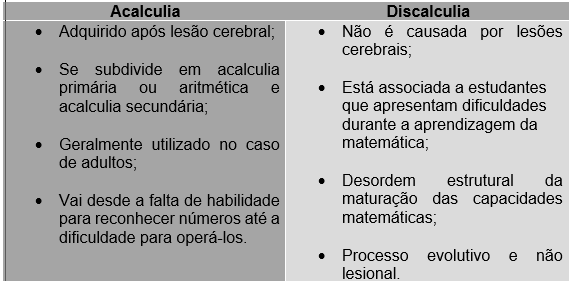
\includegraphics[width=0.95\textwidth]{diferenca_acalculia_discalculia.png} %% PARA COLOCAR O ARQUIVO DA IMAGEM NO SHARELATEX, CLIQUE NO ÍCONE QUE PARECE UMA FLECHINHA PARA CIMA (ATUALIZAR), CLIQUE EM UPLOAD E PROCURE A IMAGEM EM SEU COMPUTADOR.
\end{figure}




De acordo com \cite{Lent}, o cálculo mental matemático é de responsabilidade do hemisfério esquerdo, já o hemisfério direito é responsável pela detecção de relações espaciais quantitativas, de forma específica, no que diz respeito as relações de distância, além disso, há uma participação do hemisfério esquerdo nessa atividade através do reconhecimento das relações espaciais e qualitativas, conforme apresentado na figura 3.


\begin{figure} [hbt] 
%% hbt SIGNIFICA QUE ELE PRIMEIRO VAI TENTAR COLOCAR A IMAGEM NESTE LUGAR (h de "here"). SENÃO DER, ELE TENTA COLOCAR MAIS PRA BAIXO (b de "bottom"). SENÃO ELE COLOCA MAIS PARA CIMA (t de "top").
\label{figura1} 
%% LABEL SERVE PARA VOCÊ REFERENCIAR A FIGURA NO MEIO DO TEXTO (VEJA LINHA 330: \ref{figura1}). ASSIM VOCÊ NÃO PERDE A REFERÊNCIA QUANDO MUDA A FIGURA DE LUGAR
\caption{Funções diferenciadas dos hemisférios especializados.}
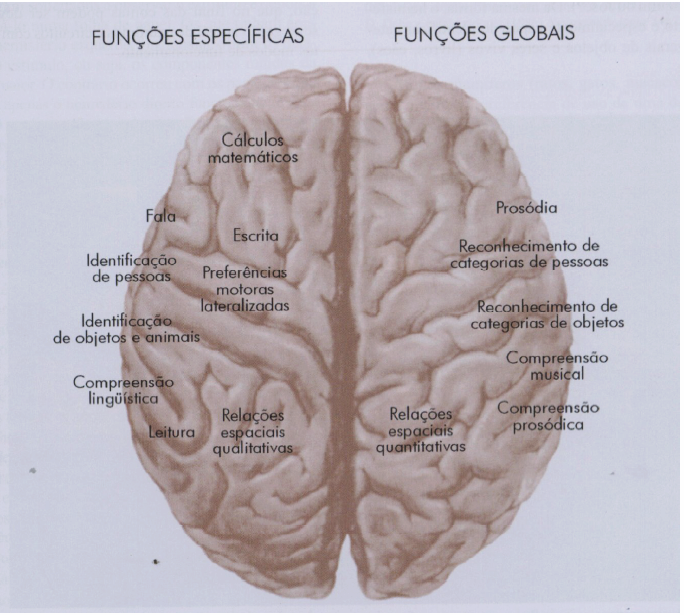
\includegraphics[width=0.95\textwidth]{cerebro.png} %% PARA COLOCAR O ARQUIVO DA IMAGEM NO SHARELATEX, CLIQUE NO ÍCONE QUE PARECE UMA FLECHINHA PARA CIMA (ATUALIZAR), CLIQUE EM UPLOAD E PROCURE A IMAGEM EM SEU COMPUTADOR.
\end{figure}



\cite{Kosk}, quando descobriu a discalculia, a classificou em 6(seis) tipos, que podem se manifestar o indivíduo de forma individual ou em conjunto. Os tipos de discalculia são:

•   Discalculia verbal - se caracteriza pela dificuldade na habilidade de nomear quantidades matemáticas, números termos e relações;

•	Discalculia Practognóstica - caracteriza-se pela dificuldade de enumerar, comparar ou manipular objetos, imaginários ou reais;

•	Discalculia Léxica - caracteriza-se pela dificuldade em ler símbolos matemáticos, problemas de cunho matemático;

•	Discalculia Gráfica - Refere-se a dificuldade na escrita dos símbolos matemáticos;

•	Discalculia Ideognóstica - refere-se a dificuldade para realizar operações mentais e para compreender os conceitos matemáticos;

•	Discalculia Operacional - dificuldade para realizar operações e cálculos matemáticos.

É importante lembrar que a discalculia pode manifestar-se em alunos que possuem capacidades em diversas áreas, mas que apresentam dificuldades com a matemática. A criança pode não se interessar pela atividade, simplesmente por não compreendê-la.

De acordo com \cite{Villar}, pesquisas apontam que a discalculia acomete cerca de 4 a 6 porcento da população mundial, nas pesquisas realizadas apenas com crianças. Tal porcentagem aponta a precisão de cuidados adequados, previnindo demais problemas.

% ---
% --- Seção dentro do capítulo
\section{Diagnóstico e Intervenção}

As dificuldades de aprendizagem geralmente, manifestam-se muito cedo na vida, não decorrem de deficiência intelectual ou de doenças adquiridas. Quase sempre tais dificuldades ocasionam muito sofrimento na vida do indivíduo, principalmente nos casos não diagnosticados. Por conta disso considera-se que o diagnóstico é um fator muito importante na dificuldade de aprendizagem, pois o diagnóstico permite que o indivíduo compreenda a razão de suas dificuldades e possa buscar ajuda especializada, a intervenção.

O diagnóstico envolve uma série de testes que podem qualificar ou quantificar as habilidades cognitivas do desenvolvimento escolar, tanto da fala, escrita, leitura e matemática esperado para a idade daquele aluno ou da escolarização, \cite{Villar}.



Caso não haja a intervenção adequada, a defasagem de desempenho escolar pode aumentar com o passar dos anos trazendo prejuízos irreparáveis como, por exemplo, o abandono escolar, dificuldade de adaptação social e baixa auto-estima, \cite{Villar}.



\begin{figure} [hbt] 
%% hbt SIGNIFICA QUE ELE PRIMEIRO VAI TENTAR COLOCAR A IMAGEM NESTE LUGAR (h de "here"). SENÃO DER, ELE TENTA COLOCAR MAIS PRA BAIXO (b de "bottom"). SENÃO ELE COLOCA MAIS PARA CIMA (t de "top").
\label{figura1} 
%% LABEL SERVE PARA VOCÊ REFERENCIAR A FIGURA NO MEIO DO TEXTO (VEJA LINHA 330: \ref{figura1}). ASSIM VOCÊ NÃO PERDE A REFERÊNCIA QUANDO MUDA A FIGURA DE LUGAR
\caption{Sintomas mais frequentes da Discalculia.}
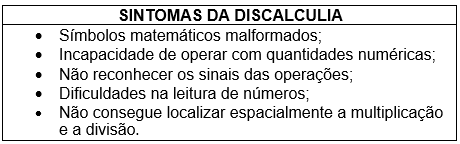
\includegraphics[width=0.95\textwidth]{tabela.png} %% PARA COLOCAR O ARQUIVO DA IMAGEM NO SHARELATEX, CLIQUE NO ÍCONE QUE PARECE UMA FLECHINHA PARA CIMA (ATUALIZAR), CLIQUE EM UPLOAD E PROCURE A IMAGEM EM SEU COMPUTADOR.
\end{figure}

A pesquisa de campo é o principal método de coleta de dados. Baseia-se no estudo de indivíduos, grupos, com o objetivo de melhor entender as diferentes características de uma determinada comunidade e realizar um levantamento de informações sobre um determinado problema. Os cinco métodos mais utilizados na coleta de informação são: questionários, entrevistas, observação direta, registros institucionais e grupos focais (BARBOSA; SILVA, 2010).

Dentre os métodos de coleta mais utilizados:

•	Questionários – consistem em um formulário, que pode ser impresso ou online, contém perguntas importantes relacionados ao tema e podem ser respondidas sem a presença de um entrevistador; fornecendo informações necessárias e diretas em uma dada pesquisa. É possível coletar informações de pessoas geograficamente distantes;

•	Entrevistas – caracterizada por uma conversa guiada por um entrevistador com um roteiro de perguntas ou tópicos, buscando obter informações do entrevistado;

•	Observação direta - é um método que pode ser definido como um acompanhamento presencial do processo a ser modelado que sujeita o pesquisador a um contato mais direto com a realidade;

•	Registros institucionais - Uma das primeiras fontes de informação a serem consideradas é a existência de registros na própria organização, sob a forma de documentos, fichas, relatórios ou arquivos em computador. O uso de registros e documentos já disponíveis reduz tempo e custo de pesquisas para avaliação;

•	Grupos focais – é o método que permite coletar informações de mais de duas pessoas simultaneamente, quando essas estão reunidas numa espécie de discussão e entrevista coletiva.


Também chamados de survey (pesquisa ampla) o questionário é uma técnica de custo razoável, apresenta as mesmas questões para todas as pessoas, garante o anonimato e pode conter questões para atender a finalidades especificas de uma pesquisa. Consiste  nas técnicas de investigação mais utilizadas nas pesquisas de campo dando liberdade aos usuários poderem responder questionários independente de restrições espaciais e temporais (OMOTE, 2005), sendo assim a técnica escolhida para a coleta de informações por atender a todos os requisitos necessários.

Os questionários podem conter perguntas abertas e fechadas. As perguntas abertas permitem ao usuário construir a resposta com as suas próprias palavras, e melhor expressar sua opinião. As perguntas fechadas são aquelas em que o usuário apenas seleciona opções (dentre um conjunto de opções apresentadas) que mais se adequem à sua opinião. Quando aparecem questões dos dois tipos no mesmo questionário, este é considerado um questionário misto (CRUZ, 2016).


% ---
% --- Seção dentro do capítulo
\section{Diagnóstico e Intervenção}
Geoprocessamento consiste em armazenar a geometria e os atributos de dados georreferenciados. Dados georreferenciados são elementos que estão localizados na superfície terrestre numa projeção cartográfica (Câmara 2005). É destinado ao processamento dos dados georreferenciados desde a sua coleta até a geração de saídas na forma de mapas convencionais, relatórios, etc. Por meio da localização e do processamento de dados geográficos, integra várias tecnologias para coleta, tratamento, análise e apresentação de informações associadas a mapas digitais georreferenciados (ROCHA, 2000).

O conjunto de tecnologias do Geoprocessamento operando sobre base de dados geocodificados ou sobre bancos de dados geográficos, executa análise, reformulações e sínteses sobre os dados disponíveis, através da coleta e tratamento de informações espaciais com determinado objetivo, executadas por sistemas específicos para cada aplicação (KRIEGER et al., 2003). 

O Geoprocessamento surgiu devido ao elevado crescimento das tecnologias de software e hardware aplicadas ao gerenciamento de informações e processamento de dados e imagens geográficas. O objetivo era automatizar parte do processamento de dados com características espaciais, diminuindo custos de produção e manutenção de mapas, principalmente quando comparados ao da produção manual, uma vez que esta emprega mídias físicas como o papel, que podem se tornar caras principalmente considerando os aspectos de armazenamento e atualização parte do processamento de dados (RECKZIEGEL, 2009).

Georreferenciamento consiste em tornar as coordenadas de dados de informação geográfica visíveis, estando relacionados a localização geográfica na superfície da terra. Podendo ser representados por uma imagem ou mapa entre outras formas onde um sistema de geoprocessamento desempenha a função de armazená-los.

\section{Tecnologia no diagnóstico}
Sistemas de Informação Geográfica são sistemas de informações construídos especialmente para armazenar, analisar e manipular dados geográficos, ou seja, dados que representam objetos e fenômenos cujo tratamento prescinde da localização geográfica. (CÂMARA, 2005). 

Os SIGs correspondem às ferramentas computacionais de Geoprocessamento, que permitem a realização de análises complexas, ao integrar dados de diversas fontes e ao criar bancos de dados georreferenciados. Burrough (1986) considera que estes sistemas não apresentam apenas a função de manipulação de dados geográficos, mas, dentro de um SIG, os dados estruturados representam um modelo do mundo real.

O SIG pode ser considerado um sistema que realiza o tratamento computacional de dados geográficos e recuperam informações, não apenas com base em suas características alfanuméricas, mas também através de sua localização espacial; oferece aos administradores e técnicos uma visão ampla do ambiente de atuação, na qual as informações disponíveis estão ao seu alcance, inter-relacionadas com base num aspecto comum que é a sua localização geográfica. 

Arquitetura de um SIG

Devido à grande procura de aplicações SIG em diversas áreas, incluindo aplicações no transporte, na agricultura, na floresta, cartografia entre outros, os SIGs podem ser utilizados de três maneiras distintas. São elas (CÂMARA, 2005).

•	Como ferramenta para produção de mapas;

•	Como suporte para análise espacial de fenômenos; 

•	Também como um banco de dados geográficos, com funções de armazenamento e recuperação de informação espacial.

A partir das definições, podemos resumir as principais características de um SIG enumeradas por Câmara (2005):

•	Integrar, numa única base de dados, as informações espaciais provenientes de dados cartográficos; e dados alfanuméricos provenientes de censo e cadastro urbano e rural, imagens de satélite, redes e modelos numéricos de terreno;

•	Oferecer mecanismos para combinar as várias informações, através de algoritmos (instruções) de manipulação e análise, bem como para consultar, recuperar, visualizar e plotar o conteúdo da base de dados georreferenciados.



Em uma visão mais ampla, a estrutura geral de um SIG (CÂMARA, 2005): 

\begin{figure} [hbt] 
%% hbt SIGNIFICA QUE ELE PRIMEIRO VAI TENTAR COLOCAR A IMAGEM NESTE LUGAR (h de "here"). SENÃO DER, ELE TENTA COLOCAR MAIS PRA BAIXO (b de "bottom"). SENÃO ELE COLOCA MAIS PARA CIMA (t de "top").
\label{figura1} 
%% LABEL SERVE PARA VOCÊ REFERENCIAR A FIGURA NO MEIO DO TEXTO (VEJA LINHA 330: \ref{figura1}). ASSIM VOCÊ NÃO PERDE A REFERÊNCIA QUANDO MUDA A FIGURA DE LUGAR
\caption{Arquitetura de um Sistema de Informação Geográfica.}
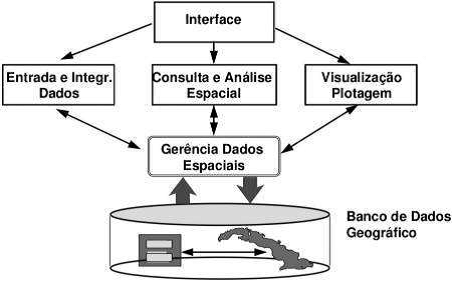
\includegraphics[width=0.95\textwidth]{arquitetura.png} %% PARA COLOCAR O ARQUIVO DA IMAGEM NO SHARELATEX, CLIQUE NO ÍCONE QUE PARECE UMA FLECHINHA PARA CIMA (ATUALIZAR), CLIQUE EM UPLOAD E PROCURE A IMAGEM EM SEU COMPUTADOR.
\end{figure}

•	Interface – a interface com o usuário contempla as diretrizes de controle e operacionalização do sistema, sendo este o nível que está mais próximo do usuário final; 

•	Entrada e integração de dados - desempenham funções de conversões dos dados geográficos para um formato adequado ao armazenamento.

•	Consulta e Análise espacial – mecanismos que permitem a realização de cálculos para obtenção de estatísticas espaciais, responsáveis por mapear essa informação no formato de saída;

•	Visualização e plotagem -  responsável pelo processamento dos dados de entrada e saída, possibilitando a edição, análise e visualização de dados;

•	Gerenciamento de dados espaciais -  corresponde ao armazenamento recuperação e gerenciamento de dados espaciais, sendo o nível mais interno do sistema.

Um SIG pode ser visto como uma representação simplificada digital das características da terra para uma determinada região. Os dados georreferenciados podem ser organizados dentro do SIG utilizando diferentes critérios, por exemplo, como camadas temáticas ou objetos espaciais (CRUZ; CAMPOS, 2005).

Em um SIG, os dados geográficos são estruturados em planos de informação, também denominados de camadas. As camadas quando estão sendo referenciadas geograficamente a algum sistema de coordenadas, sendo eles, topográficas, geográficas, geodésicas ou cartesianas podem ser sobrepostas e representam o mundo real (FRANCISCO et al.,  ). Para que ocorra a correta sobreposição, é necessário encontrar o ponto em comum entre a projeção cartográfica, sistemas de coordenadas e sistema geodésico (DATUM). O DATUM consiste em um sistema de referência e coordenadas associado a características terrestres.

\begin{figure} [hbt] 
%% hbt SIGNIFICA QUE ELE PRIMEIRO VAI TENTAR COLOCAR A IMAGEM NESTE LUGAR (h de "here"). SENÃO DER, ELE TENTA COLOCAR MAIS PRA BAIXO (b de "bottom"). SENÃO ELE COLOCA MAIS PARA CIMA (t de "top").
\label{figura1} 
%% LABEL SERVE PARA VOCÊ REFERENCIAR A FIGURA NO MEIO DO TEXTO (VEJA LINHA 330: \ref{figura1}). ASSIM VOCÊ NÃO PERDE A REFERÊNCIA QUANDO MUDA A FIGURA DE LUGAR
\caption{Representação das camadas temáticas.}
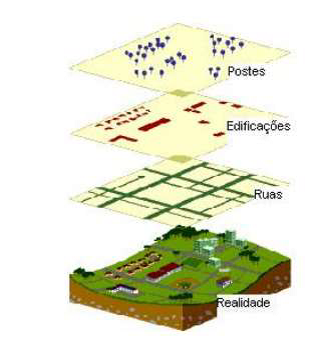
\includegraphics[width=0.95\textwidth]{camada.png} %% PARA COLOCAR O ARQUIVO DA IMAGEM NO SHARELATEX, CLIQUE NO ÍCONE QUE PARECE UMA FLECHINHA PARA CIMA (ATUALIZAR), CLIQUE EM UPLOAD E PROCURE A IMAGEM EM SEU COMPUTADOR.
\end{figure}


% ---


\begin{figure} [hbt] 
%% hbt SIGNIFICA QUE ELE PRIMEIRO VAI TENTAR COLOCAR A IMAGEM NESTE LUGAR (h de "here"). SENÃO DER, ELE TENTA COLOCAR MAIS PRA BAIXO (b de "bottom"). SENÃO ELE COLOCA MAIS PARA CIMA (t de "top").
\label{figura1} 
%% LABEL SERVE PARA VOCÊ REFERENCIAR A FIGURA NO MEIO DO TEXTO (VEJA LINHA 330: \ref{figura1}). ASSIM VOCÊ NÃO PERDE A REFERÊNCIA QUANDO MUDA A FIGURA DE LUGAR
\caption{Representação da estrutura matricial (raster)}
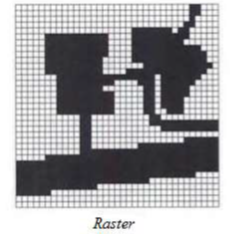
\includegraphics[width=0.45\textwidth]{raster.png} %% PARA COLOCAR O ARQUIVO DA IMAGEM NO SHARELATEX, CLIQUE NO ÍCONE QUE PARECE UMA FLECHINHA PARA CIMA (ATUALIZAR), CLIQUE EM UPLOAD E PROCURE A IMAGEM EM SEU COMPUTADOR.
\end{figure}

Nas estruturas vetoriais um número finito de segmentos em linha reta são definidos pelos seus pontos finais. A representação de um elemento ou objeto é uma tentativa de reproduzi-la o mais exatamente possível. Qualquer entidade ou elemento gráfico de um mapa é reduzido a três formas básicas: pontos, linhas ou polígonos. Caracteriza-se por ser uma representação adequada para uma ampla gama de dados espaciais sendo mais vantajoso que a matricial por armazenar pontos de interesse ao sistema (CÂMARA, 2005).

\begin{figure} [hbt] 
%% hbt SIGNIFICA QUE ELE PRIMEIRO VAI TENTAR COLOCAR A IMAGEM NESTE LUGAR (h de "here"). SENÃO DER, ELE TENTA COLOCAR MAIS PRA BAIXO (b de "bottom"). SENÃO ELE COLOCA MAIS PARA CIMA (t de "top").
\label{figura1} 
%% LABEL SERVE PARA VOCÊ REFERENCIAR A FIGURA NO MEIO DO TEXTO (VEJA LINHA 330: \ref{figura1}). ASSIM VOCÊ NÃO PERDE A REFERÊNCIA QUANDO MUDA A FIGURA DE LUGAR
\caption{Representação da estrutura vetorial}
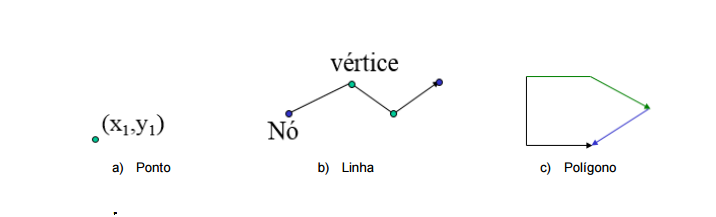
\includegraphics[width=0.95\textwidth]{vetorial.png} %% PARA COLOCAR O ARQUIVO DA IMAGEM NO SHARELATEX, CLIQUE NO ÍCONE QUE PARECE UMA FLECHINHA PARA CIMA (ATUALIZAR), CLIQUE EM UPLOAD E PROCURE A IMAGEM EM SEU COMPUTADOR.
\end{figure}

As diferenças entre os dados geográficos de estrutura vetorial e estrutura matricial são várias, como:

•	Precisão Geométrica: Os dados de estrutura vetorial possuem uma precisão geométrica maior que os dados de estrutura matricial;

•	Tamanho do arquivo: Os dados de estrutura vetorial necessitam de menor espaço em disco para serem armazenados;

•	Processamento: O processamento de dados matriciais é mais simples, os dados matriciais são indicados para o processamento de elementos da superfície contínua;

•	Exibição: Os dados de estrutura vetorial são mais rápidos para serem exibidos.

(PORQUE A ESCOLHA DO VETORIAL....)

Banco de Dados Geográficos
Os SIG precisam armazenar grandes quantidades de dados e torná-los disponíveis para operações de consultas e análise (LISBOA FILHO,). Com o aumento na procura por SIG, houve a necessidade de gerenciadores de dados geográficos que armazenam tanto a geometria como também os atributos dos objetos em um Sistemas Gerenciadores de Banco de Dados (SGBD) que são ferramentas fundamentais paro os SIG.

Os SIGs lidam com grandes quantidades de dados, e o armazenamento e manipulação desses dados tornam-se uma tarefa difícil devido à grande quantidade de informações. Desta forma, o uso de Sistemas de Gerenciamento de Banco de Dados é imprescindível na administração dessas informações.

O componente de armazenamento do SIG, denominado Banco de Dados Geográficos (BDG), estrutura e armazena os dados para possibilitar a realização das operações de análise e persistência de dados espaciais, capazes de descrever fenômenos geográficos cuja localização está relacionada a uma posição sobre a superfície terrestre (CÂMARA, 2005).
Existe um grande número de pesquisas na área de banco de dados voltadas a buscar novas formas de gerenciar dados georreferenciados. Atualmente, a estrutura mais utilizada na elaboração dos SIG é a que emprega um sistema dual. O SIG é composto de SGBD relacional, responsável pela gerência dos atributos acoplado a um componente de software responsável pelo gerenciamento dos atributos espaciais (LISBOA FILHO,).


% --- Seção dentro do capítulo


\chapter{Trabalhos Relacionados}
Existem ferramentas digitais com o propósito de aprimorar os métodos que auxiliam na coleta de dados. A ferramenta \textit{Data Goal}, trabalha com questionários digitais, enviando de imediato, se existir conexão com à Internet, os dados coletados em campo para um servidor da base de dados das entrevistas para acompanhamento em tempo real. O diferencial positivo em relação ao \textit{Data Goal} é a não depência à conexão com a \textit{Internet}.

O \textit{QuickTapSurvey}, facilita a criação de questionários e coletas de dados de forma interativa permitindo que os usuários criem seus próprios questionários e coletas de dados de forma interativa, permitindo assim, os usuários criarem seus próprios questionários e coletem respostas sem depender de conexão à Internet.

O Nokia Data Gathering é um sistema que provê a criação de questionários móveis que, colocados em um servidor na Internet, podem ser acessados pelos dispositivos móveis com acesso à rede. Os dados são coletados e armazenados nos dispostivos e podem ser transmitidos para um servidor. 

Um projeto similar que devemos citar é o Maritaca que consiste numa arquitetura de construção de aplicações para coleta de dados usando dispositivos móveis; os usuários têm a liberdade de construir seus questionários compostos por diversas perguntas. Nos dispositivos móveis, o aplicativo permite a coleta de dados utilizando interfaces amigáveis, onde os dados são armazenados nos smartphones até serem transferidos para o servidor, sem que haja conexão à internet para a coleta. Entretanto a criação fica restrita ao navegador web.

Um ponto diferencial da arquitetura proposta é a criação dos questionários customizados e a coleta é feita pela aplicação móvel, e poderá ser armazenada informações de localização geográfica; e a \textit{interfece web} será responsável por prover meio de exibição dos dados coletados e oferece mecanismos de consultas geográficas utilizando a ferramenta SIG acoplada.

Conforme observado, existem trabalhos semelhantes ao projeto que está sendo proposto. Entretanto, não tratam de todos os pontos apresentados nesta arquitetura, que tem como intuito permitir ao usuário maior capacidade de manipulação de suas informações através de diversas funcionalidades.



\chapter{Desenvolvimento da Aplicação}
A proposta desse trabalho consiste na criação de uma \textit{Interface web} para exibição e manipulação das informações geográficas, que compõe um dos quatro módulos de uma arquitetura para coleta de questionários customizados georreferenciados. Essa arquitetura é caracterizada por permitir o armazenamento da localização geográfica dos questionários coletados, a capacidade de customização das sequências de perguntas e a manipulação dos dados georreferenciados.

Os módulos da arquitetura foram assim determinados: 

•	Modelagem de um banco de dados geográficos; 

•	Desenvolvimento de uma ferramenta SIG para suporte;

•	Desenvolvimento de uma \textit{interface web} para visualização;

•	Desenvolvimento de uma aplicação móvel de coleta.


A visualização dos questionários será feita pelo SIG Web, com o propósito de exibir os dados que forem obtidos pelo aplicativo \textit{Android} nas pesquisas de campo. Essa \textit{Interface} será responsável por prover meios para visualizar a distribuição espacial destes dados, podendo realizar consultas geográficas e filtros de perguntas.

Inicialmente, para o desenvolvimento da \textit{Interface} de apresentação, foi necessária a modelagem de uma ferramenta SIG e também a modelagem e implementação do banco de dados geográficos que deu suporte à execução do projeto. 

Foram realizados testes sobre o banco de dados já implementado que envolveram a criação de questionários fictícios e realizados consultas geográficas na ferramenta SIG desenvolvida. Dessa maneira a aplicação foi desenvolvida utilizando as seguintes tecnologias:

•	Modelagem do Banco de Dados Geográfico – Foi utilizado o banco de dados PostgreSQL com a extensão espacial PostGIS. A integração do Banco de Dados (BD) com a extensão espacial acontece de forma transparente para o usuário, mas complexa internamente. O PostGIS fornece a ligação do BD com os tipos de dados espaciais, e permite o uso de objetos do SIG;

•	Ferramenta SIG – A ferramenta SIG servirá para manipular os dados geográficos que forem armazenados no banco de dados. A modelagem de teste para a ferramenta foi feita em ambiente web utilizando a linguagem de programação PHP, que é uma linguagem livre responsável pela conexão do banco de dados PostgreSQL com A API Google Maps, sendo o conteúdo e resultado dessa conexão visualizado diretamente al algum navegador. A versão utilizada do PHP foi 5.5.12 compilada com o servidor web Apache 2.4.9.

o	A API Google Maps interage com o PHP obtendo respostas da conexão usando retorno de dados. Foi a ferramenta utilizada para visualizar mapas e acessar recursos avançados de mapeamento, como exibição de polígonos, pontos, dentre outros.

o	Para aprofundar nos conhecimentos dos recursos dos SIGs, e colocar em prática na API do Google Maps, foram utilizadas algumas ferramentas de software SIG: o gvSIG e QGIS.


\section{Diagrama Entidade Relacionamento}


\begin{figure} [hbt] 
%% hbt SIGNIFICA QUE ELE PRIMEIRO VAI TENTAR COLOCAR A IMAGEM NESTE LUGAR (h de "here"). SENÃO DER, ELE TENTA COLOCAR MAIS PRA BAIXO (b de "bottom"). SENÃO ELE COLOCA MAIS PARA CIMA (t de "top").
\label{figura1} 
%% LABEL SERVE PARA VOCÊ REFERENCIAR A FIGURA NO MEIO DO TEXTO (VEJA LINHA 330: \ref{figura1}). ASSIM VOCÊ NÃO PERDE A REFERÊNCIA QUANDO MUDA A FIGURA DE LUGAR
\caption{Diagrama Entidade Relacionamento}
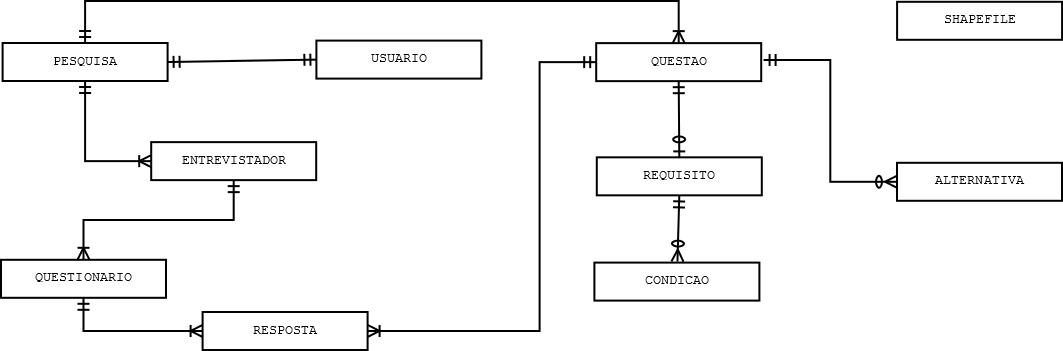
\includegraphics[width=0.95\textwidth]{diagrama.png} %% PARA COLOCAR O ARQUIVO DA IMAGEM NO SHARELATEX, CLIQUE NO ÍCONE QUE PARECE UMA FLECHINHA PARA CIMA (ATUALIZAR), CLIQUE EM UPLOAD E PROCURE A IMAGEM EM SEU COMPUTADOR.
\end{figure}

Adiante, será explicada a modelagem e tabelas utilizadas pelo sistema de questionário:

(TABELA AQUI).....

\section{Arquitetura de Coleta de Questionários}



O ponto diferencial da arquitetura para a coleta de questionários, é poder dar a liberdade para a customização de seus questionários, ou seja, definindo diferentes fluxos de sequência para as perguntas e suas distribuições espaciais. Sendo uma opção importante na aplicação de pesquisas diante diferentes perfis de usuários, tornando assim o processo flexível e levando ao foco das pergutas de interesse.


Como já mencionado a arquitetura de coleta de questionários customizados é composta por quatro módulos.

É representado na figura acima a estrutura da arquitetura. Composta por um \textbf{Banco de Dados Geográfico} que servirá como base para a implementação do projeto, e serão armazenados dados coletados dos questionários incluindo as localizações geográficas.

\textbf{A ferramenta SIG} servirá como o suporte para a arquitetura por meio de suas ferramentas para coletar, armazenar, manipular, e analisar as informações. A base de dados permitirá a interpretação segundo diferentes visões. 

A visualização dos questionários será feita pelo \textbf{SIG Web}, com o propósito de exibir os dados que forem obtidos pelo aplicativo Android nas pesquisas de campo. Essa \textit{Interface} é responsável por prover meios para visualizar a distribuição espacial destes dados, podendo realizar consultas geográficas e filtros de perguntas.

A criação dos questionários customizados será realizado por meio de um \textbf{Aplicativo} desenvolvido na plataforma \textit{Android}. A aquisição dos dados é realizada através da tecnologia do GPS, pois possibilita a realização de levantamentos de campo com alto grau de precisão sem dependência de conexão à \textit{Internet} .

\begin{figure} [hbt] 
%% hbt SIGNIFICA QUE ELE PRIMEIRO VAI TENTAR COLOCAR A IMAGEM NESTE LUGAR (h de "here"). SENÃO DER, ELE TENTA COLOCAR MAIS PRA BAIXO (b de "bottom"). SENÃO ELE COLOCA MAIS PARA CIMA (t de "top").
\label{figura1} 
%% LABEL SERVE PARA VOCÊ REFERENCIAR A FIGURA NO MEIO DO TEXTO (VEJA LINHA 330: \ref{figura1}). ASSIM VOCÊ NÃO PERDE A REFERÊNCIA QUANDO MUDA A FIGURA DE LUGAR
\caption{Estrutura da Arquiteura}
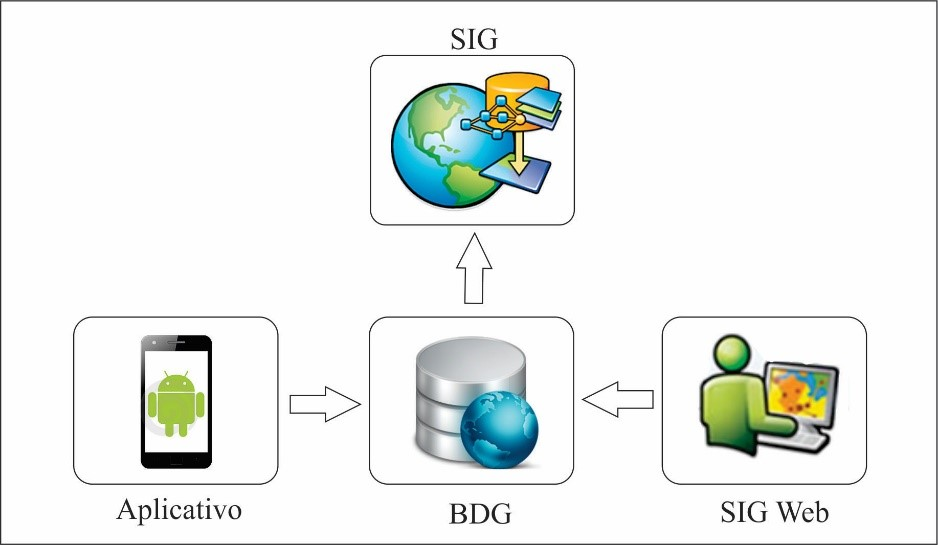
\includegraphics[width=0.95\textwidth]{arquituraproposta.jpg} %% PARA COLOCAR O ARQUIVO DA IMAGEM NO SHARELATEX, CLIQUE NO ÍCONE QUE PARECE UMA FLECHINHA PARA CIMA (ATUALIZAR), CLIQUE EM UPLOAD E PROCURE A IMAGEM EM SEU COMPUTADOR.
\end{figure}

% ---
% Conclusão
% ---
\chapter{Conclusão}

A procura por informação geoespacial cresceu bastante pela popularização dos dispositivos móveis, e com isso a evolução dos Sistemas de Informação Geográficos se tornaram mais presentes no cotidiano das pessoas.

Considerando que o propósito inicial deste trabalho consiste na criação de uma interface web de visualização dos dados georreferenciados que serão coletados por meio de uma ferramenta móvel de coleta, nota-se que foi possível obter os resultados desejados acerca da proposta.

Uma proposta de estilização de uma página web afim de levar os usuários deste projeto a uma maior comodidade para visualizar as pesquisas e questionários realizados.
Vale ressaltar que uma parte da página web já tinha sido implementada anteriormente por outro membro do projeto, pois necessitava da criação para a implantação das tecnologias SIGs aplicadas por ela. Esse trabalho consistiu na continuação do mesmo, trazendo uma fluidez à página e otimizando-a.

A Grandiosidade deste projeto e o alcance que ele pode chegar é muito positivo, pois o objetivo é dar a liberdade de que seus usuários criem as pesquisas de acordo com o interesse próprio, em suas atividades de campo, observando diretamente os fenômenos geográficos sob diferentes pontos de vista.

Os testes realizados das consultas geográficas com questionários fictícios mostraram resultados satisfatório no que se diz respeito a lógica de customização proposta pelo projeto. Mostraram eficiência e agilidades com as ferramentas espaciais, como também ao banco de dados geográficos acoplado.

Como trabalhos futuros, está planejado o desenvolvimento da aplicação do sistema Android para os dispositivos móveis, que dará suporte à coleta de questionários customizados, permitindo aos usuários a criação dos questionários e a coleta dos dados.
(INCOMPLETO).


\chapter{Publicações}
Caso o aluno possua publicações de artigos científicos, estes deverão ser listados neste capítulo.

% ----------------------------------------------------------
% ELEMENTOS PÓS-TEXTUAIS
% ----------------------------------------------------------
\postextual


% ----------------------------------------------------------
% Referências bibliográficas
% ----------------------------------------------------------
\bibliography{references} %% REFERENCIA AO ARQUIVO abntex2-modelo-references.bib

% ----------------------------------------------------------
% Glossário
% ----------------------------------------------------------
%
% Consulte o manual da classe abntex2 para orientações sobre o glossário.
%
%\glossary

% ----------------------------------------------------------
% Apêndices
% ----------------------------------------------------------

% ---
% Inicia os apêndices
% ---
\begin{apendicesenv}

% Imprime uma página indicando o início dos apêndices
\partapendices

% ----------------------------------------------------------
\chapter{Apêndice}
% ----------------------------------------------------------


\end{apendicesenv}
% ---



\end{document}
